\documentclass[border=10pt]{standalone}
\usepackage[svgnames]{xcolor}
\usepackage{amsmath}
\usepackage{pgfplots}
\pgfplotsset{compat=newest}
\usepackage[sfdefault]{FiraSans}
\usepackage{FiraMono}
\renewcommand*\familydefault{\sfdefault}
\begin{document}
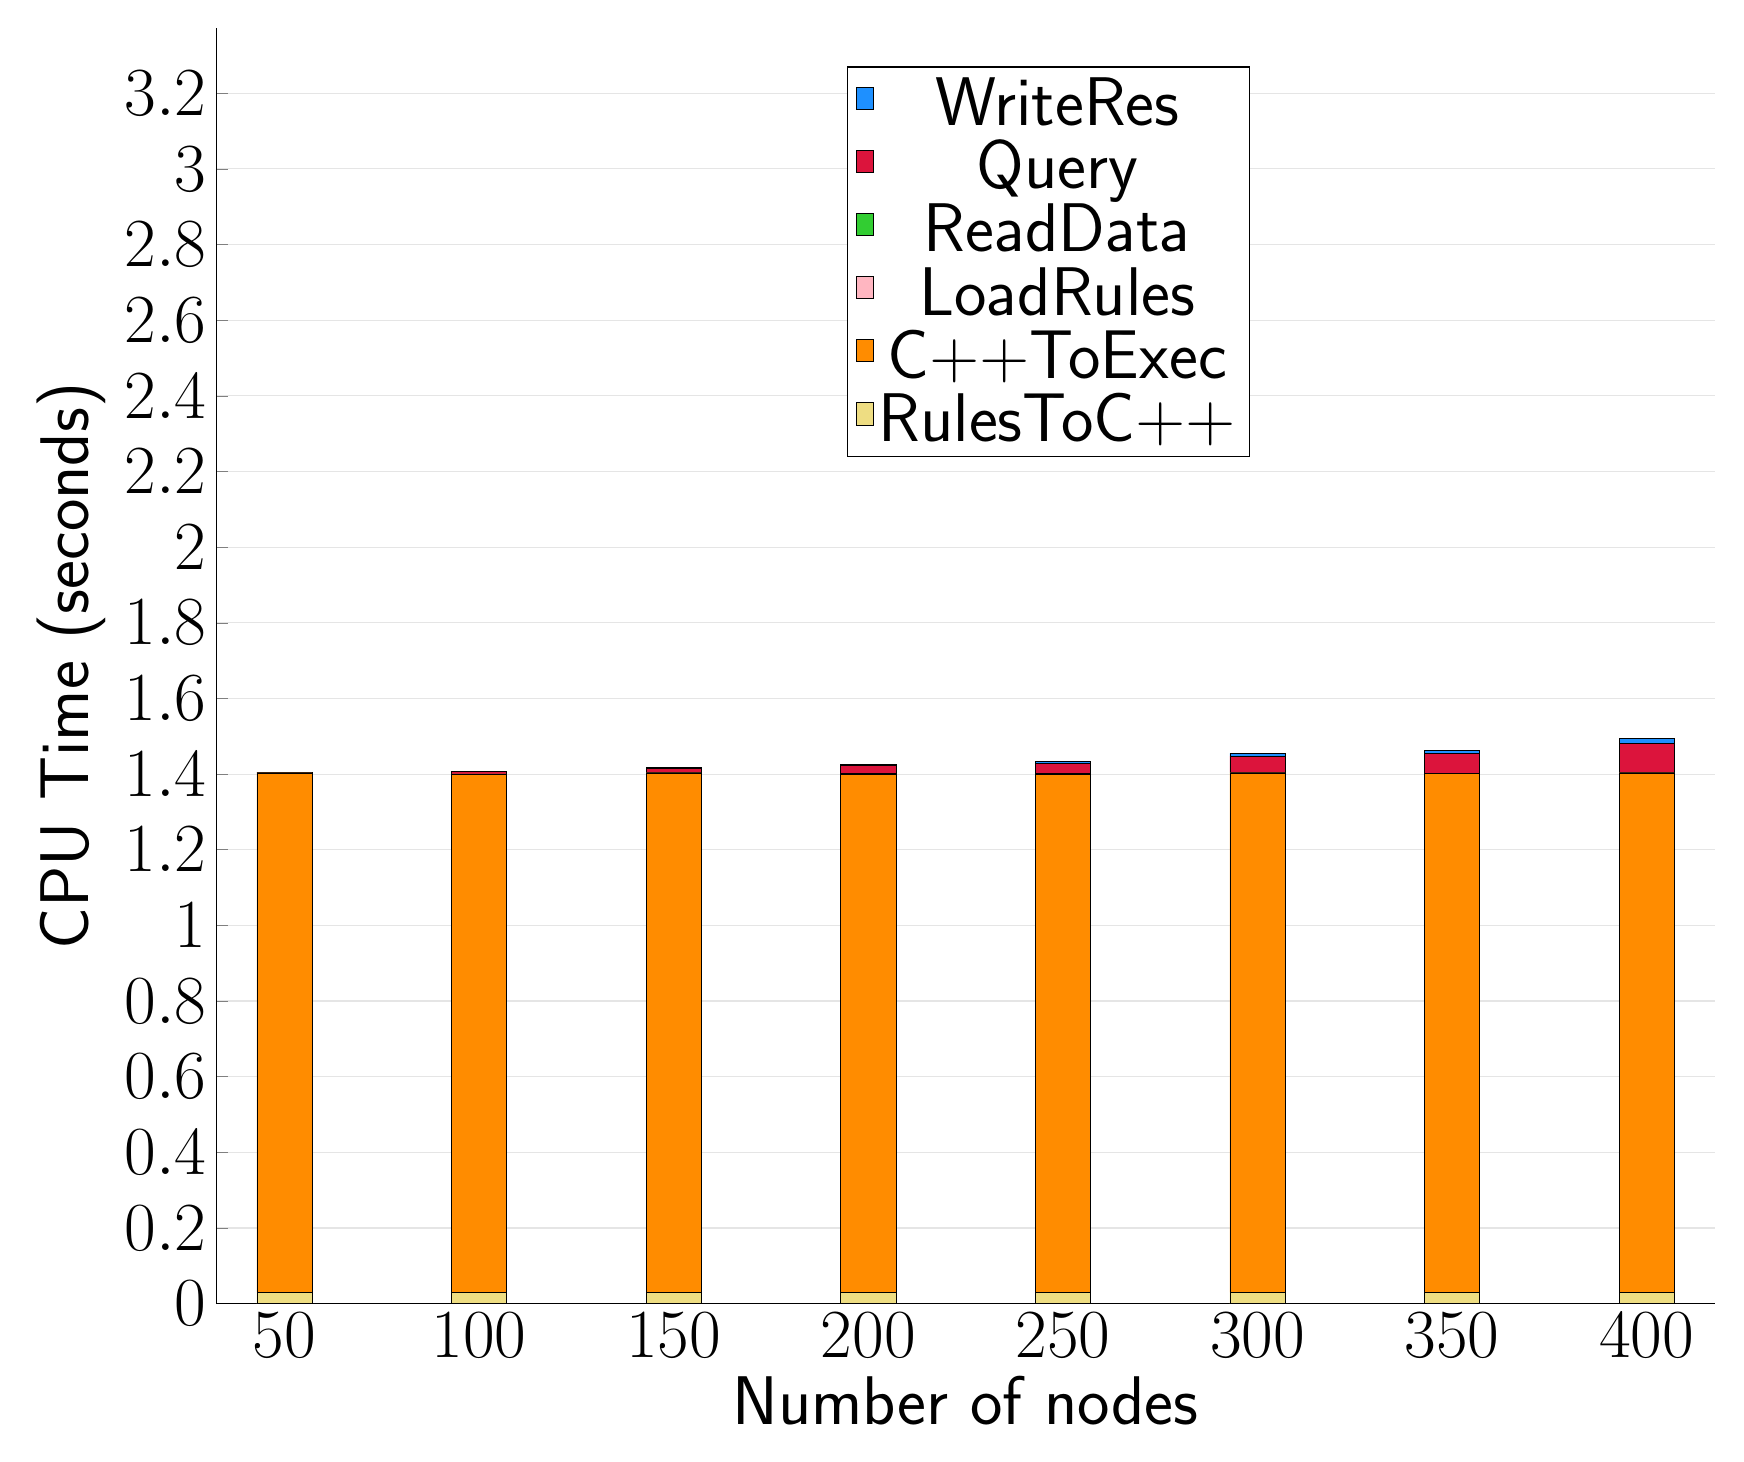
\begin{tikzpicture}
\begin{axis}[
   ybar stacked,
   width=1.7\textwidth,
   bar width=0.7cm,
   ymajorgrids, tick align=inside,
   major grid style={draw=gray!20},
   xtick=data,
   ymin=0, ymax=3.3720000000000003,
   axis x line*=bottom,
   axis y line*=left,
   enlarge x limits=0.05,
   legend style={
       at={(0.69, 0.97)},
       anchor=north east,
       legend columns=1,
       font=\Huge,
   },
   ylabel={CPU Time (seconds)},
   xlabel={Number of nodes},
   label style={font=\Huge},
   tick label style={font=\Huge},
]
\addlegendimage{fill=DodgerBlue, draw=black, line width=0.2pt}
\addlegendentry{WriteRes}
\addlegendimage{fill=Crimson, draw=black, line width=0.2pt}
\addlegendentry{Query}
\addlegendimage{fill=LimeGreen, draw=black, line width=0.2pt}
\addlegendentry{ReadData}
\addlegendimage{fill=LightPink, draw=black, line width=0.2pt}
\addlegendentry{LoadRules}
\addlegendimage{fill=DarkOrange, draw=black, line width=0.2pt}
\addlegendentry{C++ToExec}
\addlegendimage{fill=LightGoldenrod, draw=black, line width=0.2pt}
\addlegendentry{RulesToC++}
\addplot +[fill=LightGoldenrod, draw=black, line width=0.2pt] coordinates {
(50, 0.030000000000000006)
(100, 0.030000000000000006)
(150, 0.030000000000000006)
(200, 0.030000000000000006)
(250, 0.030000000000000006)
(300, 0.030000000000000006)
(350, 0.030000000000000006)
(400, 0.030000000000000006)
};
\addplot +[fill=DarkOrange, draw=black, line width=0.2pt] coordinates {
(50, 1.3730000000000002)
(100, 1.3700000000000003)
(150, 1.3730000000000004)
(200, 1.3700000000000003)
(250, 1.3700000000000003)
(300, 1.3730000000000004)
(350, 1.371)
(400, 1.373)
};
\addplot +[fill=LightPink, draw=black, line width=0.2pt] coordinates {
(50, 0.0001155)
(100, 0.0001163)
(150, 9.919999999999999e-05)
(200, 9.95e-05)
(250, 0.00011270000000000002)
(300, 0.00011279999999999999)
(350, 0.00010870000000000001)
(400, 9.2e-05)
};
\addplot +[fill=LimeGreen, draw=black, line width=0.2pt] coordinates {
(50, 0.0004068)
(100, 0.0006006)
(150, 0.0007356999999999999)
(200, 0.000959)
(250, 0.0010628999999999999)
(300, 0.0013739000000000002)
(350, 0.0014149)
(400, 0.0017656999999999998)
};
\addplot +[fill=Crimson, draw=black, line width=0.2pt] coordinates {
(50, 0.0012343)
(100, 0.005648200000000001)
(150, 0.0114977)
(200, 0.0213543)
(250, 0.027607100000000002)
(300, 0.0431208)
(350, 0.051973300000000014)
(400, 0.0771452)
};
\addplot +[fill=DodgerBlue, draw=black, line width=0.2pt] coordinates {
(50, 0.0005489000000000001)
(100, 0.0015336)
(150, 0.0027530999999999996)
(200, 0.0042326)
(250, 0.005171)
(300, 0.0073131)
(350, 0.0086033)
(400, 0.012383700000000001)
};
\end{axis}
\end{tikzpicture}

\end{document}
